\documentclass[A4,12pt]{article}
\usepackage{geometry}
\usepackage{multicol}
\usepackage{lipsum}
\usepackage{changepage}
\usepackage{graphicx}
\graphicspath{  }
\usepackage{booktabs}
\usepackage{cite}
\usepackage{float}
\usepackage{hyperref}
\usepackage[font={small,it}]{caption}
\usepackage[english]{babel}
\usepackage{fancyhdr}

\setlength{\headheight}{15pt}

\pagestyle{fancy}
\fancyhf{}
\lhead{\textbf{Version:} 2.1  \textbf{Revision:} 4/27/18}
\rhead{\thepage}
\lfoot{Sam Penders and Caleb Lindsey}
\rfoot{\textit{Mu2e: University of Minnesota}}

\renewcommand{\footrulewidth}{1pt}

\begin{document}

\begin{titlepage}
	\centering
	
\includegraphics[width=0.5\textwidth]{mu2e_logo_oval.png}\par\vspace{2cm}
	{\scshape\LARGE CO$_2$ Leak Testing of Straws \\
		Standard Operating Procedure\par}
	\vspace{3cm}
	{\Large Sam Penders\par}
    \vspace{.5cm}
    {\small Revised by Caleb Lindsey\par}
    {\small 4/27/18\par}
	\vspace{3cm}
	{\large University of Minnesota\par}
 	\vspace{.5cm}
	{\large October 27, 2017\par}
	% Bottom of the page
	\vfill
	{\href{mailto:pende061@physics.umn.edu}
    {\tt{pende061@physics.umn.edu}}\par}
	
    {\href{Linds551@umn.edu}
    {\tt{Linds551@umn.edu}}\par}
\end{titlepage}

\clearpage
\setcounter{page}{1}

\newenvironment{myitemize} %adjust item spacing in lists to make smaller
{ \begin{itemize}
    \setlength{\itemsep}{4pt}
    \setlength{\parskip}{0pt}
    \setlength{\parsep}{0pt}     }
{ \end{itemize}                  } 

\section{Goal}
All Mylar straws in the Mu2e electron tracker panels will be inflated with a mix of argon gas and CO$_2$ during the run of the experiment. Thus, our goal is to determine the leak rate of each straw before panel installation, as well as identify straws that are damaged. We strive to do this in a safe, efficient, and reproducible manner.

%-----------------------------------------------
%	EQUIPMENT
%-----------------------------------------------

\section{Equipment Used}
\begin{multicols}{2}
\begin{myitemize}
	\item Pallet with Mylar straws
	\item CO$_2$ tank with regulator attached
	\item N$_2$ tank with regulator attached
	\item CO$_2$ pressure gauge and flow meter with hose 
	\item Vacuum grease
	\item Straw end-piece hose plugs
	\item Leak test chambers
	\item Plastic straw loading tubes
	\item Magnetic grabber
	\item Arduino Unos connected to leak chambers and computer
	\item Isopropyl alcohol and paper towels
	\item Form--fitting nitrile gloves
\end{myitemize}
\end{multicols}

%-----------------------------------------------
%	RISKS AND DANGERS
%-----------------------------------------------

\section{Risks and Dangers}
There is an inherent danger when working with pressurized gases. Because the N$_2$ and CO$_2$ tanks are pressurized to a maximum of 2500 psi, an uncontrolled discharge of gas from the cylinders would effectively make the cylinders into rockets. This could happen if a cylinder is knocked over and the gas cylinder valve or regulator valve gets damaged. For this reason, compressed gas chambers are harnessed to the wall by a chain. The regulator over the exit valve limits the pressure of gas released from the chamber. To prevent accidental tipping of the cylinders, only a trained supervisor should ever move cylinders or adjust regulator pressure. 

High levels of CO$_2$ in the air can make a person feel dizzy. To CO$_2$ levels from getting high, the lab has a good ventilation system. Make sure that you can hear the sound of fans from the laboratory ventilation system when working with the CO$_2$. If you do feel dizzy, close the CO$_2$ tank valve and step outside for a few minutes. Always close the gas tanks when not in use.

Care must be taken when cleaning with isopropyl alcohol. Contact with skin can cause irritation, so nitrile gloves should be worn at all times. If alcohol gets on skin, it should be washed off with soap and water. If alcohol gets in your eyes, they should be rinsed in the eye wash for several minutes. Then, go to a doctor.


\newpage

\section{Leak Testing Procedure}

\subsection{Setup}
\begin{enumerate}
	\item Put on nitrile gloves that fit snuggly. These must be worn at all times when handling straws.
	\item Check that the regulator is attached to CO$_2$ tank. Do not touch center regulator knob. Open both the gas cylinder and regulator exit valve completely. (Figure \ref{co2tank}) If these are only partially opened, gas may leak from the valve.   
	\item Check cylinder pressure. If below 200 psi, stop using cylinder immediately. If below 500 psi, have Dan order a new cylinder.
	\item Adjust flow meter on near pressure gauge to 10 scfh. Cover end of CO$_2$ nozzle with finger and confirm that the pressure on near pressure gauge reads $15.0 \pm 0.1$ psi. If not, consult a supervisor.
\end{enumerate}

\begin{figure}
	\center
	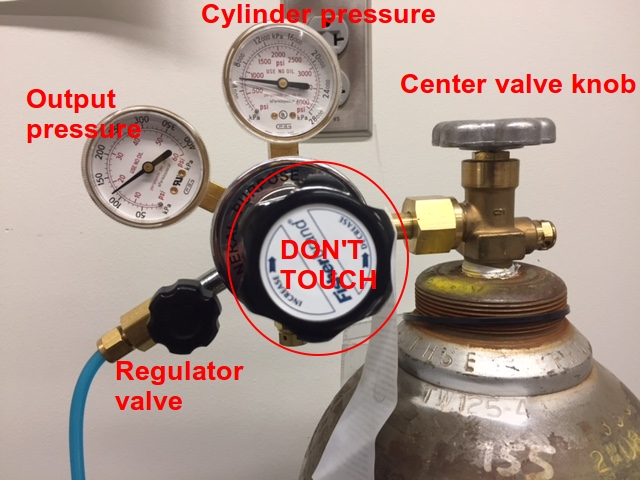
\includegraphics[scale=0.5]{co2tank}
	\caption{CO$_2$ tank with regulator attached. The regulator adjustment knob in the center should not be adjusted. The N$_2$ tank regulator is identical.} \label{co2tank}
\end{figure}


    
    


\subsection{Loading Straws} \label{performing test}
	\begin{enumerate}
		\item On N$_2$ tank, open center and regulator valves by a full turn. Make sure N$_2$ valve is closed on each leak chamber.
		\item Insert nozzle into straw end-piece hose and let flush for 10 seconds. Meanwhile, apply a dab of vacuum grease to a hose plug, and plug hose on side opposite to CO$_2$ nozzle. \label{1}
		\item Apply dab of vacuum grease to another plug. On CO$_2$ hose side of straw, pinch end-piece hose with pliers and remove CO$_2$ hose. While continuing to pinch hose, insert plug into straw hose.
		\item If testing entire pallet, inflate all straws and then carry loaded pallet over to loading station.  For individual straws, slide inflated straw into a tube and skip to step \ref{load}.
		\item Carefully lift each straw from one end and push it into a tube about 5 inches.  Then pull the tube over the straw so that each straw is inside a tube and still on the pallet.
        \item Make sure leak chambers are empty before sliding in tubes.  Load desired straws into chambers. \label{load}
		\item With straw in chamber and the chamber open, open black N$_2$ valve lever on chamber so it will flush.  Flush chamber for about 30 seconds.  Flush only one chamber at a time. \label{flush}
		\item After flushing, close black N$_2$ valve and seal chamber by turning the white lever to the left.  
        
\end{enumerate}

\subsection{Measuring Leak Rate}
	\begin{enumerate}
    	\item Open the leak test GUI, titled "Leak Test GUI Launcher.py".  It is located on the desktop.  A picture of the right-half of the GUI is shown in figure \ref{GUI}.
        \item Before loading or unloading straws, log into the worker portal.  Do this by clicking the "log in" button at the top of the GUI and entering your worker ID.
        \item Make sure straws have been properly loaded into the chambers, following section \ref{performing test}.  Nitrogen supply should be cut off and the white lever should be closed.
        \item To start taking data on a specific row, click the "Start Data" button below the desired chamber row.  When a chamber row is active the square in which the number resides will turn green.
        \item To load each straw, click "Load Straw", enter the straw ID, and click ok.
        \item Straws take 60-90 minutes to test.  A plot of the measured data can be viewed for each straw by clicking the "Plot" icon below each straw.  This can be used to make sure straw leak rates are being measured correctly.  A proper plot will have a strong linear trend.
        \end{enumerate}

\begin{figure}
	\center
	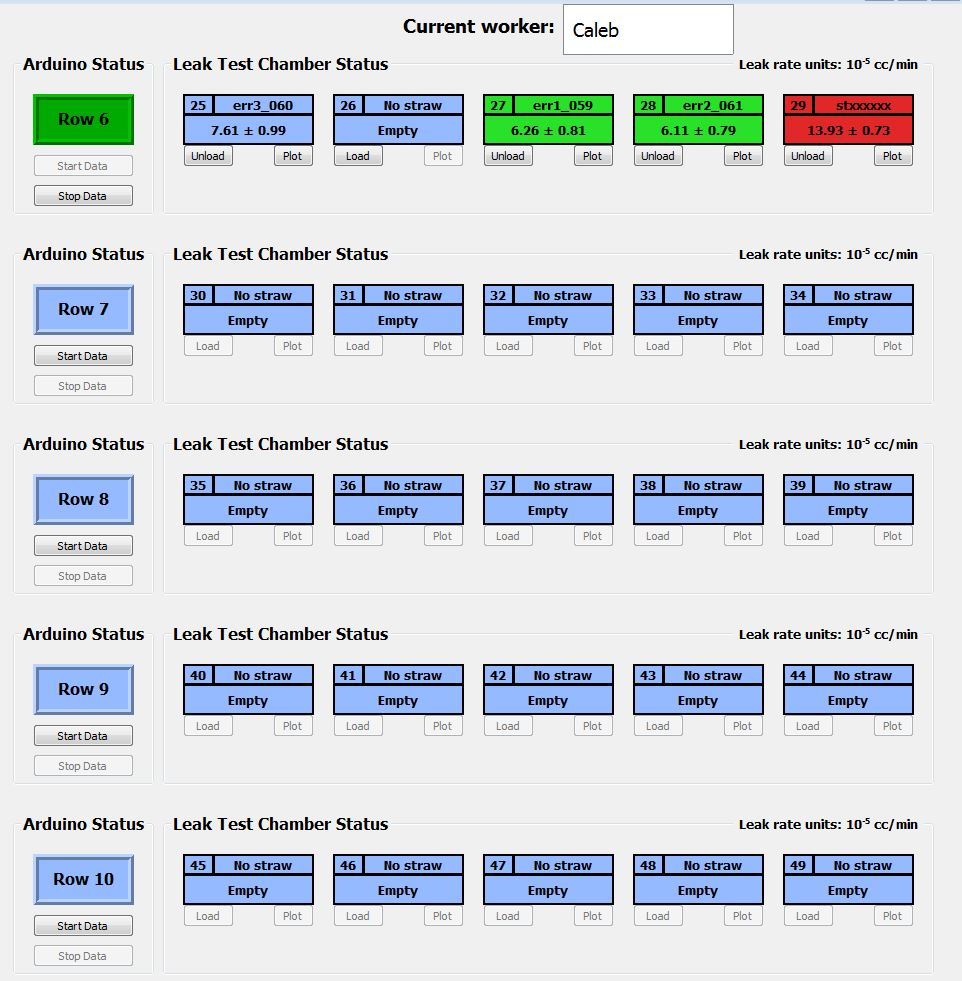
\includegraphics[scale=0.5]{GUI.JPG}
	\caption{Right-half of the Leak Test GUI.  Row 6 is the only row running.  The straws with green backgrounds pass, the red one has failed, and the blue ones are either empty or still testing.} \label{GUI}
\end{figure}






\subsection{Emptying Leak Chamber}
	\begin{enumerate}
		\item When a straw is done testing it will light up either red or green.  Green straws meet the minimum leak rate requirement, but red ones have failed.  
	\item Before physically removing finished straws, click "Unload", and make sure the straw name disappears from the GUI.  
	\item Open the white lever and use the magnetic grabber to gently remove the tube.  Slide the straw out of the tube.  Pick up straw by gently pulling straw hoses taut. Put straw back into spot on pallet.  Pull hose plugs out of straw.  
	\item If a row has no straws being tested, click "Stop Data" to turn it off.
    \item Repeat x21000
	
\end{enumerate}

\subsection{Cleanup}
	\begin{enumerate}
		\item Make sure that N$_2$ and CO$_2$ cylinder and regulator valves are closed.
		\item Put any extra straw end-piece hose plugs back into their container.
		\item Wipe and clean any vacuum grease off of work surface with alcohol and paper towel.
		\item Throw away gloves|they likely have vacuum grease on them.
	\end{enumerate}



\section{Troubleshooting}

\begin{itemize}
	\item {\bf Problem:} One of the chambers isn't taking data.
		\begin{adjustwidth}{1cm}{}
		{\bf Solution:} Make sure that the sensor cable is attached to the chamber, and is plugged securely into its Arduino port. If this doesn't work, sometimes the CO$_2$ level offset can be initially to low in the chamber. Open the straw loading valve and exhale for about half a second into chamber, then close valve. If this does not help, unplug Arduino from power supply for a minute. Then replug and try again. If the problem persists, ask for help.
		\end{adjustwidth}
\item {\bf Problem:} A straw is stuck in the chamber.
		\begin{adjustwidth}{1cm}{}
		{\bf Solution:} Unplug sensor cable from chamber, and slide entire chamber off of rack. With the straw loading valve open and hold over valve, tip chamber upside down and try to shake straw out. If this doesn't work, try to grab onto the straw with claw grabber. If this doesn't work, consult manager.
		\end{adjustwidth}
        \item {\bf Problem:} Starting a row causes the GUI to crash
		\begin{adjustwidth}{1cm}{}
		{\bf Solution:} Likely an arduino error.  Make sure the sensor cable is securely connected to the arduino port.  If it is, unplug the arduino for 30 seconds and plug it back in.
		\end{adjustwidth}
        \item {\bf Problem:} The straw I entered disappeared from the GUI
		\begin{adjustwidth}{1cm}{}
		{\bf Solution:} The program is likely still collecting data, but the straw information is not showing up.  Click "Load" and enter the straw ID again.  The straw information should return right away.  If not, ask a manager for help.
		\end{adjustwidth}
	\item {\bf Problem:} I accidentally entered the wrong straw for a chamber.
		\begin{adjustwidth}{1cm}{}
		{\bf Solution:} Empty the chamber in the program. Ask a manager to delete the incorrectly named file. Re-enter the correct straw in the leak test program.
		\end{adjustwidth}
\newpage		
\item {\bf Problem:} A straw is epoxied at the end-piece to the pallet, so I can't remove it.
		\begin{adjustwidth}{1cm}{}
		{\bf Solution:} Carefully try to peel stuck end off of plastic. If it looks okay, leak test it as usual. If it is obviously damaged, cut damaged end off of straw and give to epoxy station to re-epoxy and end-piece in.
		\end{adjustwidth}
		
\item {\bf Problem:} A straw is stuck in the chamber.
		\begin{adjustwidth}{1cm}{}
		{\bf Solution:} Unplug sensor cable from chamber, and slide entire chamber off of rack. With the straw loading valve open and hold over valve, tip chamber upside down and try to shake straw out. If this doesn't work, try to grab onto the straw with claw grabber. If this doesn't work, consult manager.
		\end{adjustwidth}
		

\end{itemize}











\end{document}
